\documentclass[conference]{IEEEtran}

% Settings
\IEEEoverridecommandlockouts
\usepackage{cite}
\usepackage{amsmath,amssymb,amsfonts}
\usepackage{algorithmic}
\usepackage{graphicx}
\usepackage{textcomp}
\usepackage{xcolor}
\usepackage[hyphens,spaces,obeyspaces]{url}
\usepackage[colorlinks,allcolors=blue]{hyperref}

\graphicspath{ {../images/} }

\def\BibTeX{{\rm B\kern-.05em{\sc i\kern-.025em b}\kern-.08em
    T\kern-.1667em\lower.7ex\hbox{E}\kern-.125emX}}

\begin{document}

% Info

\title{Plant pathlology detection with convolutional neural networks\\ }

\author{
    \IEEEauthorblockN{Barış Deniz Sağlam}
    \IEEEauthorblockA{
        \textit{Informatics Institute} \\
        \textit{Middle East Technical University} \\
        Ankara, Turkey \\
        e155841@metu.edu.tr
    }
}

% Paper

\maketitle

\begin{abstract}
\end{abstract}

\begin{IEEEkeywords}
Deep Learning, CNN, Plant Pathology
\end{IEEEkeywords}

\section{Introduction}

Apple industry in U.S. has \$15 billion annual market size \cite{Thapa2020}. 
Various kinds of plant diseases cause significant economic losses. 
The manual diagnosis of apple plant diseases are laborous and expensive. 
Hence, computer vision-based methods have been developed to detect diseases from the images of leaves. 
The variations in imaging conditions such as backgrounds, lighting, and the large variety of visual symptoms are the main challenging aspects for these methods. 

In this paper, we investigate the performance of convolutional neural networks on detecting 
plant diseases from the images of apple leaves.

\subsection{Dataset}
We use \href{https://www.kaggle.com/c/plant-pathology-2021-fgvc8/overview}{Plant Pathology 2021-FGVC8 dataset} for training the models. 
The dataset consist of over $18,632$ RGB images, 
varying between $2592 \times 1728$ to $5184 \times 3456$ in size, 
and their labels. Each sample is labelled by experts with one or more disease types 
due to the fact that a plant may have multiple diseases. 

There are 5 kinds of plant disease existing in the dataset:
\begin{enumerate}
\item \textit{frog\_eye\_leaf\_spot}
\item \textit{powdery\_mildew}
\item \textit{rust}
\item \textit{scab}
\end{enumerate}

A sample is labelled as \textit{healthy} when no disease is spotted, 
and labelled as \textit{complex} when many diseases are spotted.

\begin{figure}
    \centerline{\includegraphics[width = 0.45 \textwidth]{samples-4x4.png}}
    \caption{Sample images and labels from the dataset}
    \label{fig:samples}
\end{figure}

As it can be seen from Fig.~\ref{fig:label-dist}., there is imbalance among labels in the dataset.

\begin{figure}
    \centerline{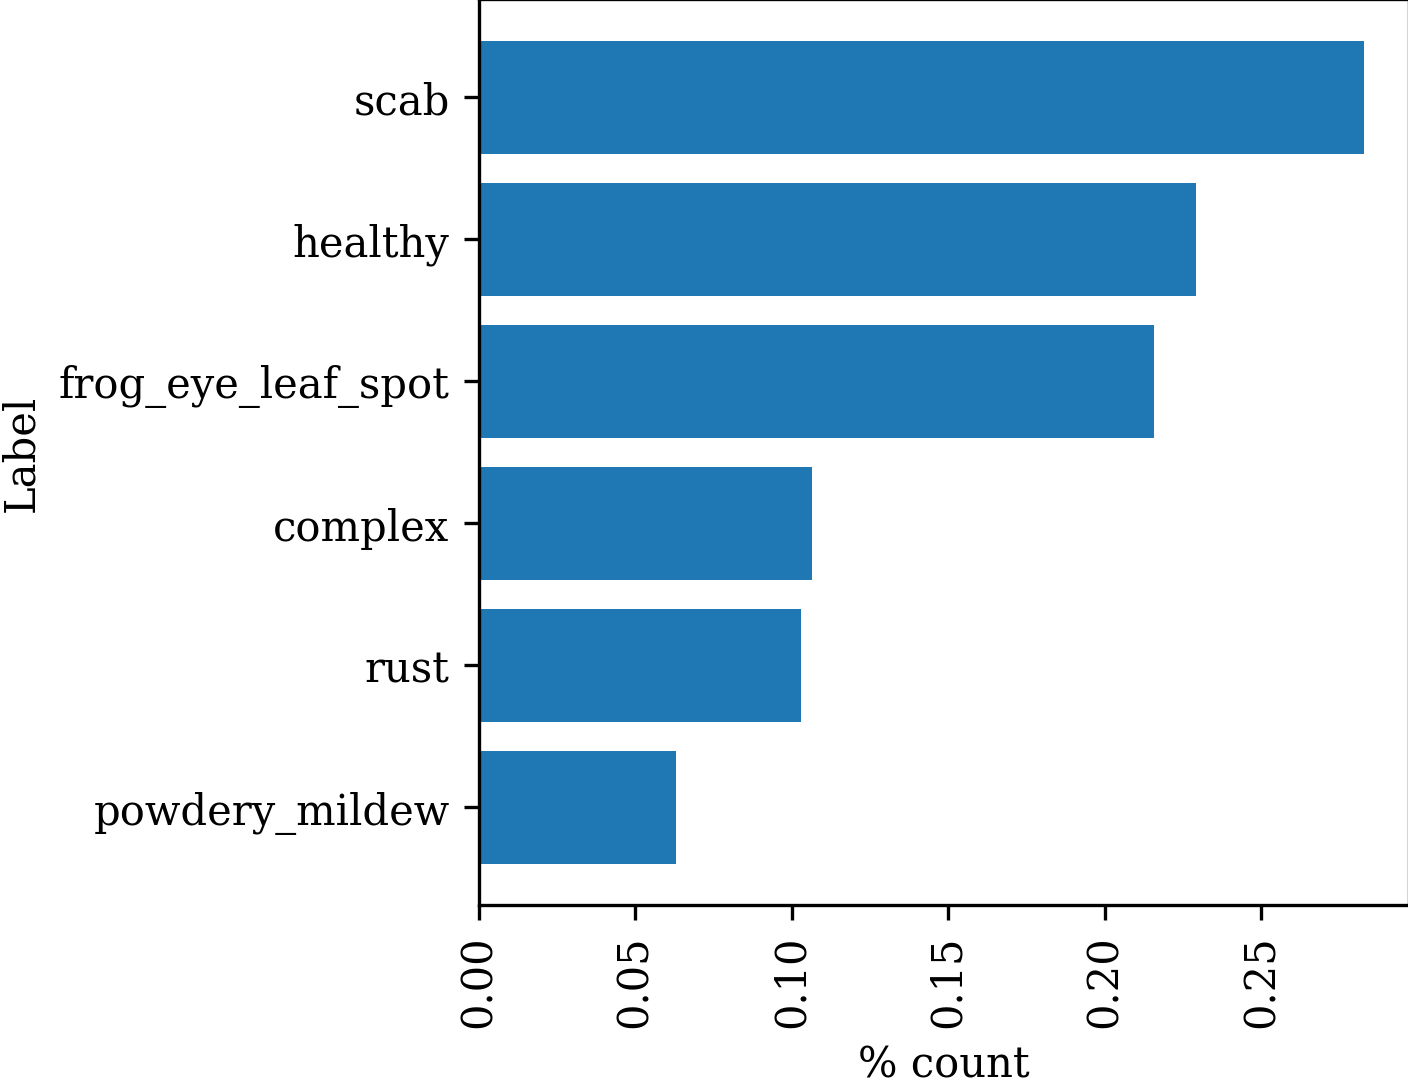
\includegraphics[width = 0.45 \textwidth]{label-dist-ratio.png}}
    \caption{Label distribution in the dataset}
    \label{fig:label-dist}
\end{figure}


\subsection{Literature Search}

\section{Methods}

\subsection{Data quality}

\subsection{Model training and evaluation}


\section{Conclusion}

\bibliographystyle{IEEEtran}
\bibliography{bibliography.bib}

\end{document}
